Теория игр - это раздел математики, изучающий оптимальные стратегии в жизненных ситуациях. Теория игр широко применима в экономике \cite{baron1989bargaining},социальных науках \cite{arrow2012social} и медицине \cite{segev2005kidney}.


Постановки выделяются поиском форм гармонического существования общества, экономическим урегулированием нежелательного поведения.

Цель работы - найти оптимальную форму аукциона в сфере образования постановки. 

Задача работы - исключить нежелательное поведения поставщиков в аукционах. К такому поведению относится:
\begin{itemize}
    \item Сговор между участниками аукциона;
    \item Инсайдерская торговля;
    \item Влияние долговой нагрузки.
\end{itemize}


\begin{figure}[h]
    \centering
    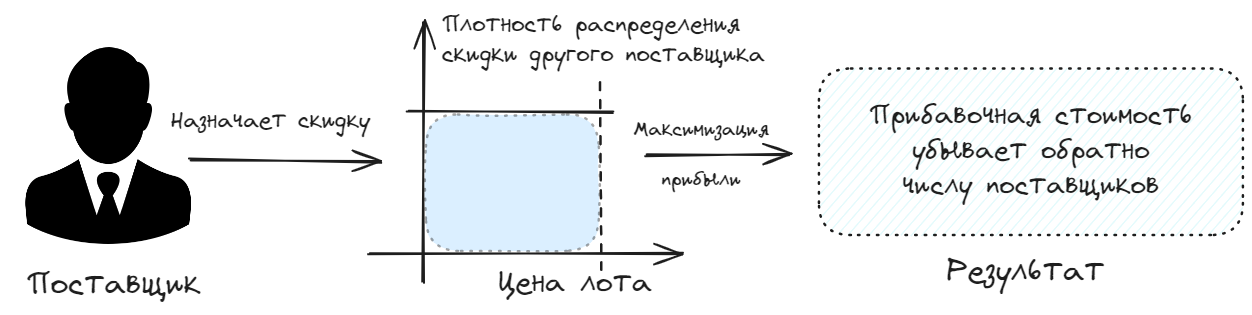
\includegraphics[width=0.5\textwidth]{assets/settings/auction_goal.excalidraw.png}
    \caption{Аукцион}
\end{figure}

Дополнительно были исследованы модели разделов для анализа бюджетного распределения.

Для выполнения поставленных целей автор разделил описание на тематические главы. В первой главе представлен обзор предметного языка, описаны экономические постановки, которые имеют развитое представление в теории игр.
В главе 2 описаны основные теоремы и математический аппарат теории игр, который используется для поиска оптимальных моделей реальных задач. В главе 3 приведено полное описание хода работ.

 
 



 